%%%% Class %%%%

% Class of the document: KOMA Script Article
%   Options: 12 points font, A4 paper, bibliography in ToC
\documentclass[a4paper,fontsize=11pt,bibliography=totoc]{scrartcl}

%%%% Preamble %%%%
% Packages inclusions
%\usepackage[top=0.75in,bottom=0.8in,left=0.75in,right=0.75in]{geometry}								% Custom margins (comment out if not needed)
\usepackage[english]{babel}				% Language settings
\usepackage{lmodern}					% Use Latin Modern font
\usepackage[nointegrals]{wasysym}
\usepackage{microtype}					% Enhanced typesetting (better reading)
\usepackage{graphicx}					% Enhanced graphics processing
\usepackage{url}
\usepackage{breakurl}
\usepackage[table,hyperref,x11names,svgnames]{xcolor}				% Allows coloring tables
\usepackage[section]{placeins}			% Ensure float elems. inside their section
\usepackage{booktabs}					% Beautiful, "pro" tables
\usepackage{adjustbox}					% Boxing capabilities for images and text
\usepackage{multirow}					% Enables tabular cells spanning multiple rows
\usepackage{array}					% Enables custom table column defintions
\usepackage[toc,page]{appendix}			% Appendices title customisation
\usepackage{enumitem}					% Customized enumerations and itemizes
\usepackage[version=3]{mhchem}			% Allows inclusion of chemical formulas and eq.
\usepackage{amssymb}
\usepackage[ruled,vlined]{algorithm2e} % Algorithms and pseudocode
\usepackage{todonotes}					% Useful to put TODO side notes
\usepackage[noblocks]{authblk}			% Allows authors with affiliations
\usepackage{lastpage}					% Allows referencing the last page
\usepackage[style=british]{csquotes}    % Allows block quotations
\usepackage{titlesec}
\usepackage{nameref}	% Allows references by name ("Section 5" vs "Conclusions")
\usepackage{fancyhdr}					% Fancy headers and footers
\usepackage{multicol}
\usepackage{pdflscape}
\usepackage{lipsum}
\usepackage[
	backend=biber,
	natbib=true,
	bibstyle=authoryear,
	citestyle=authoryear,
	sorting=nyt,
	block=space,
	hyperref=true,
	dashed=false
]{biblatex}
\usepackage{hyperref}
\hypersetup{
  unicode=true,
 	pdfpagemode={UseOutlines},
 	pdfstartview={FitV},
	bookmarks=true,
	bookmarksopen=true,
	bookmarksopenlevel=0,
	bookmarksnumbered=true,
	breaklinks=true, % to have links breaking among lines
	hypertexnames=true,
	plainpages=false,
	hidelinks=false,
	colorlinks=true,
	citecolor=Turquoise4,
	filecolor=black,
	linkcolor=DeepSkyBlue4,
	urlcolor=RoyalBlue3,
	anchorcolor=RoyalBlue3
}

% Command definitions
\makeatletter

% useful cross referencing commands
\newcommand{\fref}[1]{Figure~\ref{#1}}
\newcommand{\tref}[1]{Table~\ref{#1}}
\newcommand{\eref}[1]{Equation~\ref{#1}}
\newcommand{\cref}[1]{Chapter~\ref{#1}}
\newcommand{\sref}[1]{Section~\ref{#1}}
\newcommand{\aref}[1]{Appendix~\ref{#1}}
\newcommand{\alref}[1]{Algorithm~\ref{#1}}
\newcommand{\procref}[1]{Procedure~\ref{#1}}

\newcommand\frontmatter{%
	\cleardoublepage
	\pagenumbering{roman}}

\newcommand\mainmatter{%
	\cleardoublepage
	\pagenumbering{arabic}}

\newcommand\backmatter{%
	\cleardoublepage
}

\renewcommand\Authands{ and }

\newcommand{\norm}[1]{\lvert #1 \rvert}

\newcommand{\titlemake}[2]{%
		\begin{center}
			\parbox{#1\linewidth}{\centering\Large\sffamily\bfseries{#2}}
		\end{center}
}

\newcommand{\subtitlemake}[1]{%
	\begin{center}
		\begingroup
			\large\sffamily{#1}
		\endgroup
	\end{center}
}

\newcommand{\old}[1]{\textcolor{Red2}{#1}}

\makeatother

\newenvironment{dispositionlist}{%
	\begingroup
	\small
	\begin{enumerate}[label*=\arabic*.]
}{ %
	\end{enumerate}
	\endgroup
}

\newenvironment{checklist}{%
  \begin{list}{}{}% whatever you want the list to be
  \let\olditem\item
  \renewcommand\item{\olditem[$\Box$] }
  \newcommand\checkeditem{\olditem[$\CheckedBox$] }
}{%
  \end{list}
}

% Koma Script font modifications
\setkomafont{author}{\small}
\setkomafont{date}{\scshape}
\addtokomafont{section}{\large}
\addtokomafont{subsection}{\normalsize}
\addtokomafont{subsubsection}{\small}
\addtokomafont{caption}{\small}
\setlength{\abovecaptionskip}{2pt plus 0pt minus 2pt}
\setlist{nosep}
\renewcommand*{\bibfont}{\footnotesize}

% Formatting for paragraphs (indentation and space after par.)
\setlength{\parskip}{0.5\baselineskip}%
\setlength{\parindent}{1em}%

% Column separation
\setlength{\columnsep}{1.5em}

% Reduce space after sections
\titlespacing{\section}{0pt}{-0.25\parskip}{-0.5\parskip}
\titlespacing{\subsection}{0pt}{-0.25\parskip}{-0.6\parskip}
\titlespacing{\subsubsection}{0pt}{-0.5\parskip}{-0.75\parskip}

% Configuration of the blockquotes paragraphs
\SetBlockThreshold{0} % all blockquotes of 1 or more lines are treated as blocks

\addbibresource{references.bib}

%%%% Document %%%%

\begin{document}
% Page style set to fancy to get customized headers
\pagestyle{fancy}
\fancyhf{} % clear header and footer
\rhead{\footnotesize \today}
\lhead{\footnotesize David Martínez Rodríguez}
\chead{\footnotesize MSc Thesis - Planning Report}
\rfoot{\footnotesize \thepage}

\titlemake{0.9}{ % \titlemake[2] is a custom command -- look in the preface!
Assessing transition-oriented planning in sustainable mobility policies: a System Dynamics approach
}

\section{Background and problem description}
\label{s:background}
% The section should describe the subject matter, clarify the issues and reasons for your choice of research topic.
Transport related airborne pollution is one of the main causes of respiratory diseases and associated increase in morbidity in densely populated areas~\parencite{vimercati2011_Trafficrelatedair,who2006_Airqualityguidelines}. The link from air pollution to both severe health problems and high traffic volumes is well known and thoroughly researched~\parencite{who2006_Airqualityguidelines}. However, an unsustainable transportation system not only causes health issues, but also massive costs in terms of reduced productivity, freight delay, increased energy and fuel consumption or vehicle losses and damages, for example~\parencite{li-zeng2012_SocialCostTraffic}. The impacts of transportation and, particularly, urban mobility range from environmental pollution and its effects on human health and ecosystem stability to social and economic costs, as has been reviewed. Therefore, there is an urgent need for change in the mobility system, towards sustainable solutions that reduce the pressures on the environment and society.

To address all these issues, policy packages or simultaneous enforcing of different policies are needed, because of the complexity involved in effectively reducing mobility impacts~\parencite[ch. 3, p. 45]{garciasierra2014_Travelbehaviourenvironmental}. However, regulation cannot be designed without evaluating the caused impacts --- too many resources and possible negative outcomes would be at stake. Policy assessment from the systems thinking perspective is, thus, a key issue to develop, due to the difficulty of dealing with entire systems, their internal dynamics and the emergent systemic behaviour patterns, such as feedback loops, rebound effects and hidden causalities. In this regard, the field of System Dynamics can help capture such structures and cause-effect chains \parencite{hjorth2006_Navigatingtowardssustainable}. The holistic nature of system dynamics models can also help achieving an integrated assessment framework for urban mobility policies, by delivering information on a set of several indicators, at the environmental, social and economic levels.

On the other hand, policy development in the field of transportation has been mainly focused on two paths, according to \textcite{koehler2009_transitionsmodelsustainable}: (a) efficiency increasing measures, through incentives for technological enhancements (e.g. better engines or fuel mixes) and more stringent pollution limits and (b) behavioural change management, i.e., measures aimed at modal shift --- encouraging people to shift from private cars to public transport, for example. Both approaches, albeit successful to some extent, have not delivered the expected results so far, due to the high inertia and stabilisation mechanisms inherent to the current dominant regime for transportation: internal combustion engines cars-based mobility. Social backlash from abrupt changes, as well as industrial pressure to maintain support for the current business/social model are among the reasons for the partial success of mobility policies, with technological niches such as electric vehicles still not sufficiently developed or economically viable for the majority of the population \parencite{geels2012_AutomobilityTransitionSocio,nykvist2008_multilevelanalysis}.

However, a third way is possible, when it comes to policy design for sustainable mobility: transition management oriented policy. Its approach entails adopting a longer term thinking mindset (usually one or several generations), multi-level and multi-domain thinking, maintaining support for a large set of solutions and with a focus in system \textit{innovation} alongside system improvements \parencite{rotmans2001_Moreevolutionthan}. Moreover, flexibility in the objectives of policies is encouraged, as well as a more qualitative perspective to policy goals. All these characteristics configure a policy design mindset that could be the key to unlock a true game change in urban mobility, by drifting the focus from efficiency measures to a transition and innovation vision, where something more than technological progress is harnessed to achieve a sustainable transport system in the future.

\section{Purpose and definitions}
\colorbox{red}{!!!!TODO!!!!}
% Summarize and clarify the problem description. This will usually be done in discussion with your industrial supervisor. However, it is your responsibility to ensure that the purpose of the project is clear and well formulated. In some cases, the employer’s formulation of the mission can be shown separately. Consider carefully how much you think you have time for and which tasks take priority.
As much as holistic evaluation frameworks are needed to assess the reduction or increase in impacts resulting from the mobility system, policy makers should also focus on the transition management perspective of said policies. In order to understand the status of the system with regards to a sustainable transition, an assessment of the current and future policies is needed.

The research question that the thesis addresses is: \textit{``Can transition oriented policies trigger better system responses than traditional policy design (system efficiency and behavioural measures), when aiming for a more sustainable urban mobility system?''}

In order to answer the previous research question, an aim is set for the thesis: \textit{``To explore a method for system-wide evaluation of urban mobility policies, with regards to environmental, social and economic impacts, used in the assessment of transition oriented and traditional mobility policies''}.

The set of objectives designed to fulfil the aim of the thesis are:
\begin{enumerate}[label=(\alph*)]
	\item \textit{Identify} the important variables, impacts and system structures affecting mobility in urban areas, as well as the drivers and locking mechanisms of a potential transition towards a more sustainable transport system.
	\item \textit{Design} a conceptual model for the mobility system, including the previously identified social, environmental, economic and structural aspects.
	\item \textit{Quantify} the relations of the conceptual model to enable a more in-depth policy analysis, with respect to impact assessment.
	\item \textit{Validate} the model by performing tests to increase the confidence level of the model, as suggested by \textcite{forrester1978_TestsBuildingConfidence,qudrat-ullah2010_Howdostructural}.
	\item Carry on a \textit{case study}, reviewing and assessing mobility policies under the perspective of transition management theory, to understand the differences and potential for improvement in mobility policy design.
\end{enumerate}

\section{Method description}
\colorbox{red}{!!!!TODO!!!!}
% Discuss the options available and the choice of methodology you intend to follow. Illustrate how the method you have chosen best allows you to fulfill the purpose of the project.
The chosen tool for the conceptual modelling step is the \textit{causal loop diagram} (CLD), probably followed by \textit{system dynamics} modelling in the quantification step, although this is still not clear\footnote{The final decision between implementing the quantification step through \textit{system dynamics} or \textit{agent-based modelling} will be based on literature research and a thorough justification of the strengths and weaknesses of each method.}. The models obtained using this technique are easy to understand by a majority of stakeholders, they quickly convey the interrelations of the main components of a (dynamic) system and, finally, they are useful to highlight the feedback structure of the modelled system~\parencite{ghosh2015_DynamicSystemsEveryone}. A more detailed plan of the methodology is depicted in the following enumeration:
%
\begin{enumerate}[label=(\alph*)]
	\item Design a \textit{conceptual CLD}, linking different components in the transport system. To achieve a highly comprehensive model, iteratively expand the system boundaries of the CLD by including other aspects that affect or are affected by the transport system, with the insights provided by the literature research. The necessary data and knowledge about the diverse transportation system components will be collected on the basis of a \textit{literature review}.
	\item Using the previously gathered information and complementing it with appropriate quantitative data, fit as many \textit{equations} as possible for the links in the CLD model. The quantification is done in three steps:
	\begin{enumerate}[label=\roman*.]
		\item Identify and define the quantifiable links between \textit{core components} of the system.
		\item Quantify ``external'' links dealing with social issues, such as healthcare or accident costs, if enough data is available.
		\item Quantify the links from the core components of the system to the transition management assessment level.
	\end{enumerate}
	\item Validate the evaluation model through a set of structural, behavioural (model behaviour) and policy implication tests, dealing with sensitivity, adequacy and consistency.
	\item Evaluate a series of mobility policies, with respect to the expected impacts and transition potential through a \textit{case study} in Barcelona, assessing the city's mobility plan.
\end{enumerate}

\section{Disposition}
The preliminary document structure for the thesis report is based on a traditional research outline, due to the investigative nature of the thesis. The proposed disposition is:

\begin{dispositionlist}
	\item Introduction
		\begin{dispositionlist}
			\item Background
			\item Aim and objectives
		\end{dispositionlist}
	\item Methods
		\begin{dispositionlist}
			\item Methodological framework
			\item Causal Loop Diagrams
			\item System Dynamics modelling
			\item Transition Management assessment
		\end{dispositionlist}
	\item Results
		\begin{dispositionlist}
			\item The conceptual model
			\item The System Dynamics model
			\item Mobility plan assessment
		\end{dispositionlist}
	\item Discussion
		\begin{dispositionlist}
			\item Model calibration and limitations
			\item Transition management for mobility policies
		\end{dispositionlist}
	\item Conclusions
\end{dispositionlist}

\section{Detailed schedule}
A detailed version of the proposed thesis schedule can be seen in \fref{f:gantt} and \tref{t:schedule}. The phases that were outlined in the Thesis Synopsis document have been broken down into more specific tasks, which amount the same number of work days as the preliminary suggestion. The most important changes are:
%
\begin{itemize}
\item The model development phase (PH2) is now split up between a conceptual modelling task and a quantitative modelling one. Iterations in the conceptual mapping step will be used to develop the environmental, social and economic modules of the CLD model. The quantitative modelling phase is also split between the identification of stock and flow variables and the quantification of the dynamics of such.
\item The model benchmarking phase (PH3) consists of a model formal validation step and a case application, in which a policy framework will be assessed using the developed model.
\end{itemize}

\begin{table}[h!]
\centering
\footnotesize
\caption{Thesis scheduled \textit{phases}. Note that subtasks are not shown, but can be seen at the Gantt chart presented in \fref{f:gantt}.}
\label{t:schedule}
\begin{tabular}{lllll}
\toprule
Task & Objective & Start date & End date & Duration (work)\textsuperscript{1} \\
\midrule
PH0 Thesis definition & -- & Jan 16 & Jan 20 & 5 d \\
PH1A Literature review & (a) & Jan 23 & Feb 3 & 10 d \\
PH1B Planning report writing & -- & Jan 30 & Feb 3 & 5 d \\
Planning report & -- & Feb 3 & Feb 3 & Milestone \\
PH2 Model development & (b), (c) & Feb 6 & Mar 31 & 40d \\
PH3 Model benchmark & (d) & Apr 3 & Apr 28 & 20 d \\
PH4 Report writing & -- & May 1 & May 26 & 20 d \\
Thesis report & -- & May 26 & May 26 & Milestone \\
PH5 Presentation preparation & -- & May 29 & Jun 6 & 7 d \\
Final presentation & -- & Jun 6 & Jun 6 & Milestone \\
\bottomrule
\end{tabular}
{\\ \scriptsize \parbox{0.7\linewidth}{\textsuperscript{1} Only \textit{work} days are included in the duration specification -- weekends are excluded from the calculation. Therefore, 20 days correspond to 4 full weeks (a month) worth of work.}}
\end{table}

\begin{landscape}
\begin{figure}
\centering
{\setlength{\fboxsep}{0pt}\fbox{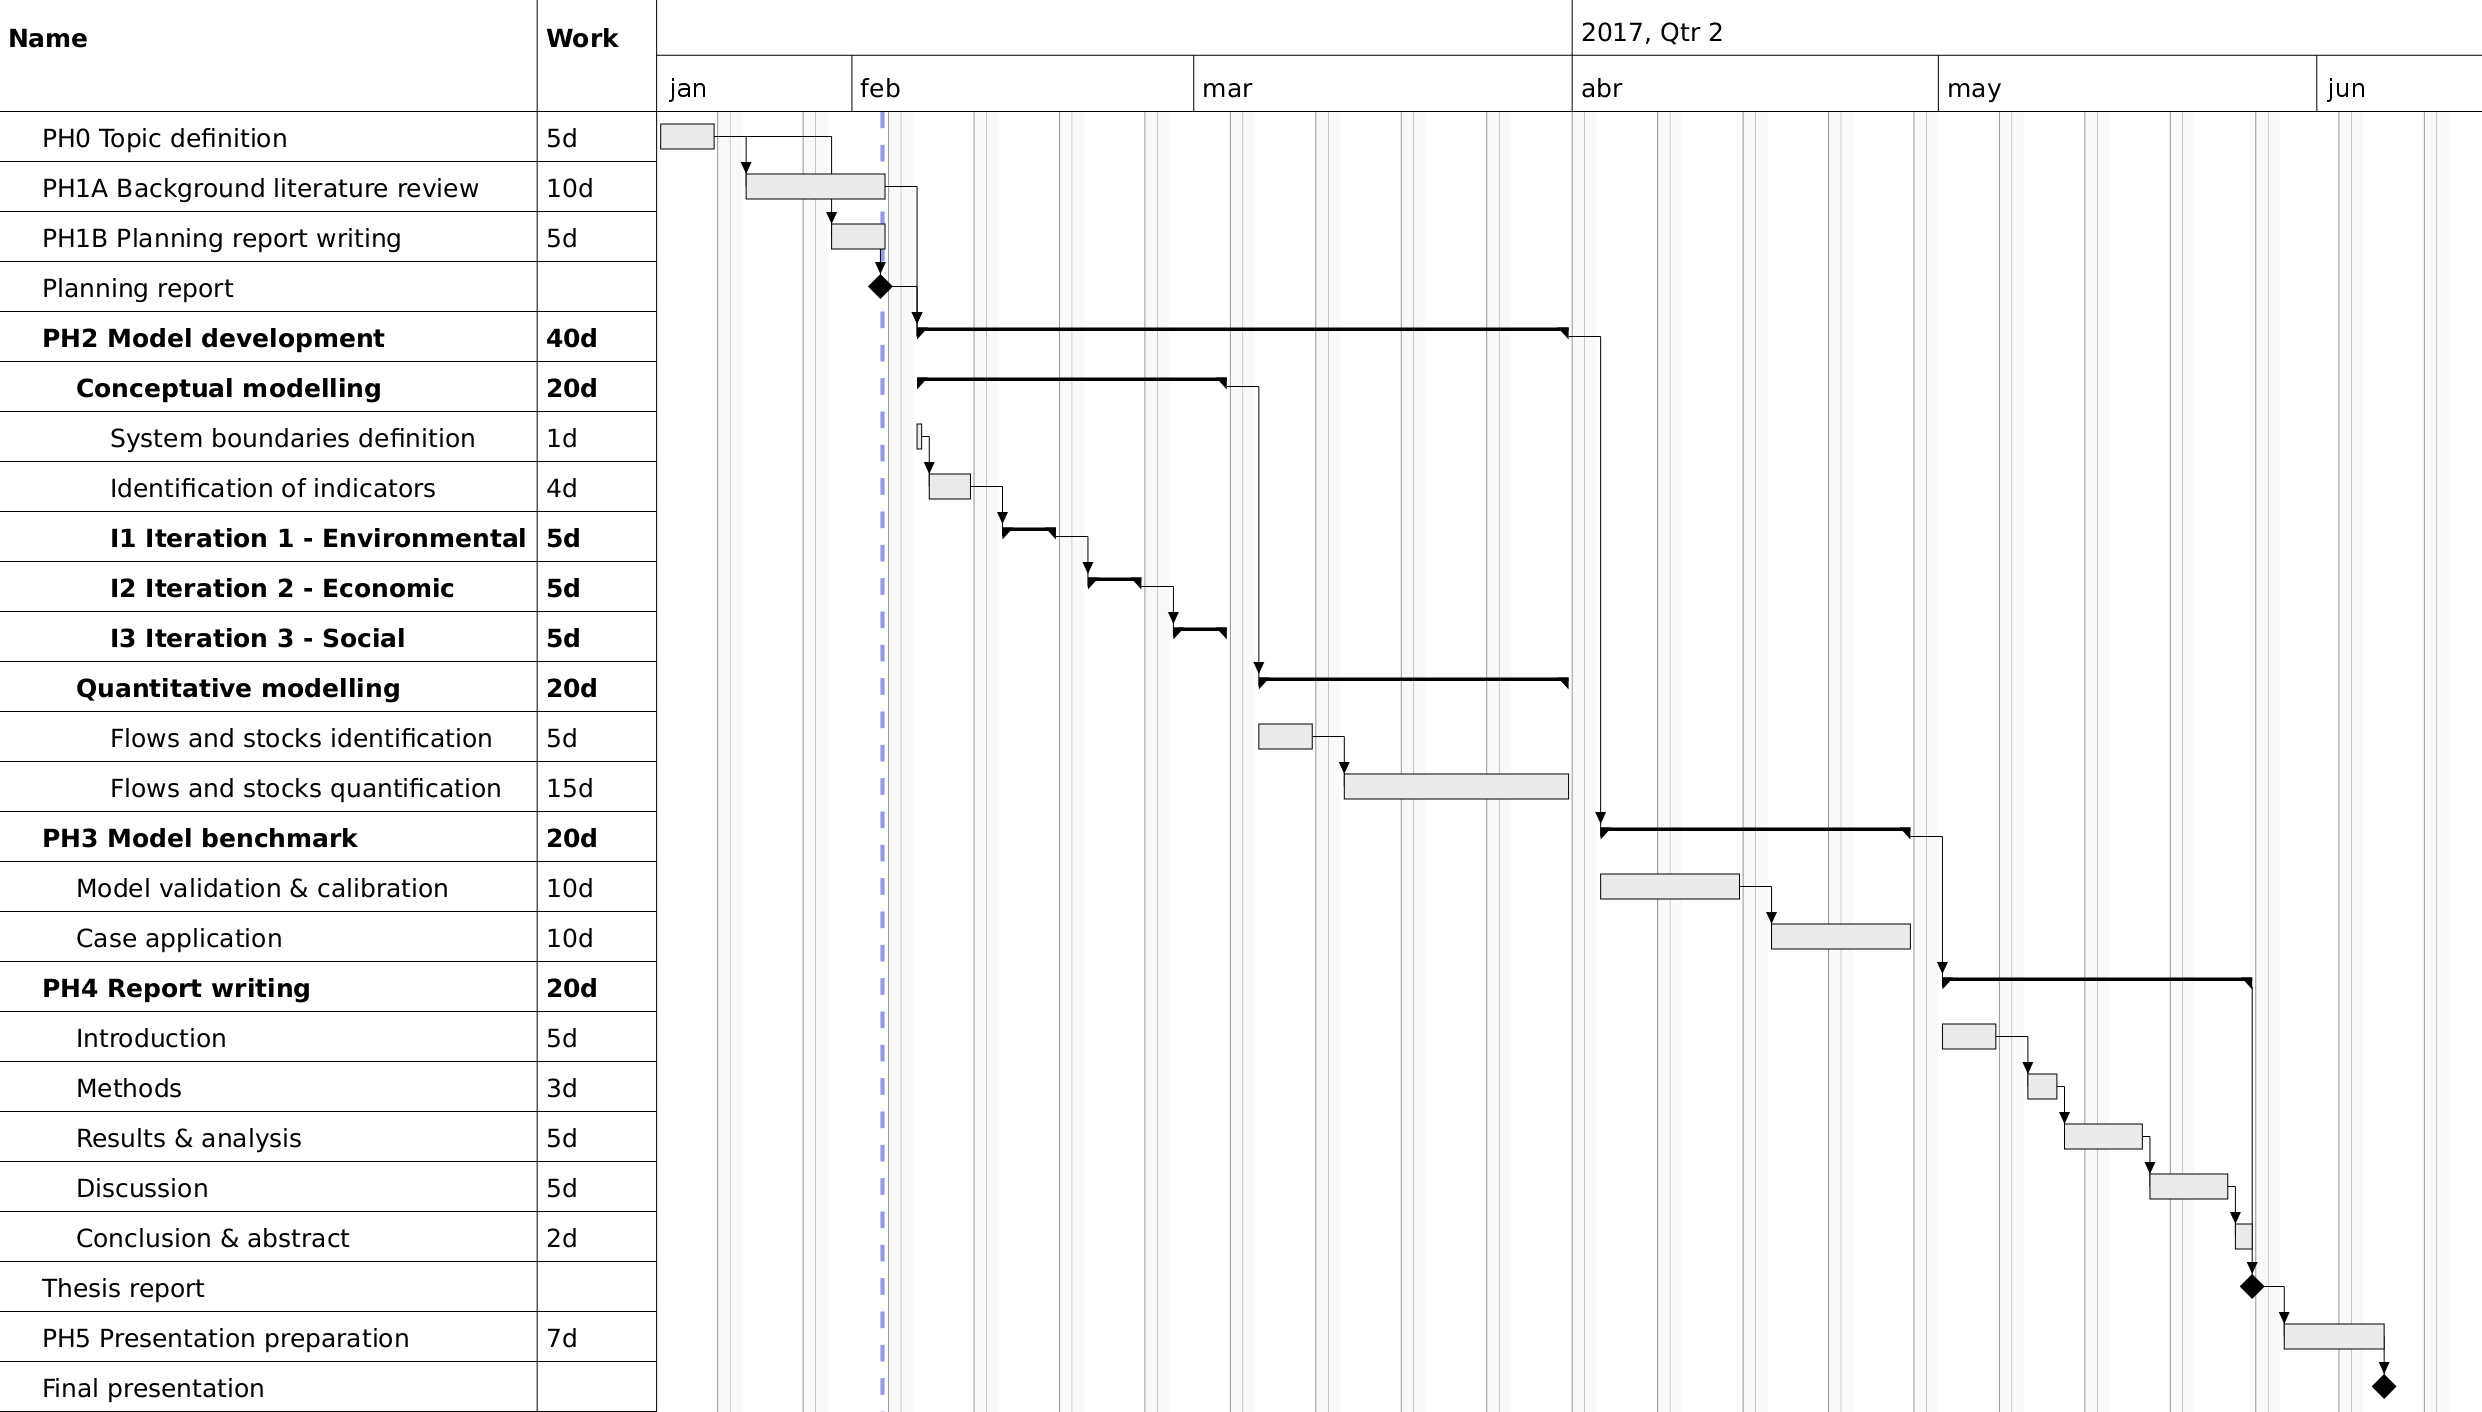
\includegraphics[width=\linewidth]{figures/thesis-gantt_complete.png}}}
\caption{Detailed Gantt chart of the thesis schedule. Milestones are marked with a $\blacklozenge$ symbol.}
\label{f:gantt}
\end{figure}
\end{landscape}

\section{Risk analysis}
% You should do a simple risk analysis of your project, as follows: "Brainstorm" all possible risks. Assess how likely it is that they will occur (rank them on a scale of 1, 3, 9, where 1 is a bit unlikely and 9 are very likely). Consider then how serious the consequences are for each risk (on a scale of 1, 3, 9). Make an action plan for those risks with the highest likelihood and/or consequence
\colorbox{red}{!!!!TODO!!!!}
Several risks have been identified with respect to the proposed thesis, considering the chosen methodology and objectives. The list of risks is presented in \tref{t:risks}, where a subjective likelihood level indicator (with possible values: 1, 3, 9) is included, as well as a summary of the consequences of incurring in every detailed risk. Alternative action plans are also included in the table, which would be put in place if the thesis project was deviating from its normal course due to any of the identified risks.

\begin{table}
	\begin{tabular}{l}
	\toprule
	Lorem ipsum\\
	\bottomrule
	\end{tabular}
\label{t:risks}
\end{table}

\printbibliography

\end{document}
